В наши дни, когда компьютерные технологии бурно развиваются, не
всегда удается создать сложное приложение, используя один язык
программирования. Разные языки имеют свои преимущества и недостатки и как
правило, что ни один из них не удовлетворят требованиям разрабатываемой
прикладной программы. Выходом из такого положения является использование
нескольких языков программирования. Такой подход часто используется при
создании программ для научных исследований, управления производственными
процессами и других коммерческих приложений. При этом приходится решать
задачи взаимодействия компонентов, написанных, которые написаны на на
разных языках программирования. Компоненты, реализующие графический
интерфейс пользователя, управление базами данных, получение и обработку
данных в реальном времени, как правило интегрируются в одно приложение.

Для реализации поставленной задачи исследования в магистерской
диссертации был выбран пакет моделирования процессов столкновения элементарных частиц при высоких энергиях на ускорителях элементарных частиц \textit{PYTHIA} на языке программирования \textit{С++}, а также принято решение о реализации всего программного
комплекса на языке программирования \textit{Java}.
В качестве веб интерфейса был использован фреймворк \textit{Angular} на языке программирования \textit{JavaScript} и бибилотека \textit{d3} для отрисовки графиков.

\begin{figure}
	\centering
	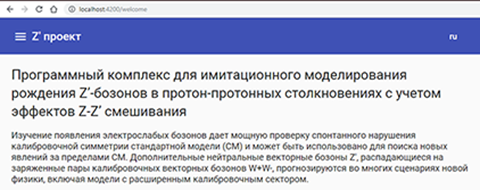
\includegraphics[width=\textwidth]{figures/welcome-page.png}
	\caption{Кварки}
	\label{fig:welcome-page}
\end{figure}
